\documentclass[12pt,a4	]{report}
\usepackage[french]{babel}
\usepackage[usenames,dvipsnames]{color}
\usepackage[utf8]{inputenc}
\usepackage{textcomp}
\usepackage[T1]{fontenc}
\usepackage{lmodern}	
\usepackage{bibunits} 
\usepackage{graphicx}
\usepackage{wrapfig}
\usepackage{float}
\usepackage{cite}
\usepackage{caption}
\usepackage{amsmath,mathtools}
\usepackage{subcaption}
\begin{document} 
\author{Moncef BEN RAJEB} 
\title{Annotation Temporelle Des Données DBpedia} 
\date{Mars 2014} 
\maketitle
\section*{Introduction générale}
\paragraph{}
Depuis la création du web il y a de cela vingt-cinq ans déjà, ce monde virtuel a vécu une évolution constante. Il offre une multitude de services aux utilisateurs individuels, aux entreprises, mais aussi à la société. Au fil des années, plusieurs versions du web ont vu le jour : le web documentaire, le web applicatif, le web social, le web mobile, etc...
\subparagraph{}
Dans le contexte de l’évolution du web une nouvelle version dite le web sémantique et sociale qui vise à propager nos modèles et leurs logiques; s’apprête à avoir le jour. Il y a plusieurs facettes du web, et le web sémantique offre un élément de réponse à l’intégration de chacune de ces facettes. Il propose d’utiliser des métadonnées pour annoter les ressources du web, et d’exploiter la sémantique des schémas de ces annotations pour les traiter avec intelligence.
\subparagraph{}
Le domaine du web sémantique est un objet de recherche sur les métadonnées du web. L'objectif principale de la naissance du web sémantique c'est d’en avoir une nouvelle version du web bien structurée qui soit capable d’en assurer le contrôle efficace des métadonnées. Dans ce contexte, DBpedia\footnote{http://dbpedia.org/About} est une base de donnée structurée qui contient des informations extraites de Wikipedia\footnote{http://wikipedia.org} et rend ces informations disponibles sur le web.
\subparagraph{}
Aussi, Resource Description Framework (RDF) est le premier des standards de la web sémantique et se trouve être un modèle à plusieurs syntaxes, dans une est  “Turtle”\footnote{http://www.w3.org/TeamSubmission/turtle/} pour publier des données à thèmes variés sur le web.
\subparagraph{}
Ce langage de modélisation permet à quiconque de décrire des ressources sur le web et aussi des ressources du web. Dans ce modèle connu comme étant la “lingua franca” du web, tout est exprimé sous forme de triplets $(subject, predicate, object)$ où chaque triplet contribue à une description du monde.
\paragraph{}
Néanmoins, des faits tels que ceux donnés dans DBpedia sont en mesure d’être adaptés au changement perpétuel du monde.
RDF n’est pas bien équipé pour exprimer d’une manière cohérente la validité temporelle des états, tels que “Obama est le président des États-Unis depuis 2008”. 
\subparagraph{}
Pour surmonter ce problème avec une modélisation RDF adéquate, plusieurs anciens travaux de recherches ont proposé d’attacher à ces triplets des annotations temporelles, ceci revient à une formalisation de ces états avec des contraintes temporelles comme des quadruplets de la manière suivante $(subject, perdicate, object, time)$ à la place du formalisme de triplet habituel.
\subparagraph{}
La théorie derrière un modèle de données basé sur des quadruplets évolue autour des termes de représentation, de connaissance, de raisonnement mais aussi d’interrogation. Or, le problème c’est qu’ils ne donnent aucune indication sur la façon dont les annotations temporelles sont créées.
\paragraph{}
De ce fait, l’objectif de ce stage est d’une part, l’extraction des informations temporelles depuis les différents documents en utilisant les techniques de fouille de données et d’autre part, d’annoter ces ressources selon leurs contextes, tout ceci mettre ces informations sous forme de quadruplets structurés dans BDpedia.
\newpage
\section*{Portée du document }
\paragraph{}
Ce mémoire de master résume les recherches, réflexions, modélisations, propositions et développements réalisés durant ce stage. Il conclut la seconde année de master Web Intelligence. Le contenu est organisé de la manière suivante :
\begin{itemize}
\item Une première partie présente l’état de l’art réalisé sur l’annotation temporelle des triplets RDF dans les bases de connaissances.
\item La deuxième partie englobe les diverses propositions pour répondre au besoins identifiés.
\item La troisième partie développe l’aspect technique de la mise en oeuvre.
\item La quatrième partie ouvre des perspectives.
\end{itemize}
\section*{État de l'art}
\subsection*{Apperçu du domaine}
\paragraph{}
Notre étude a la particulatrité de s'étandre sur le domaine de la fouille de donnée et du web sémantique.
\subparagraph{}
En effet, on va utiliser les téchniques de la fouille pour l'extraction des données dans les différents documents, et le web sémantique pour avoir une structure plus lisible par la machine.
\subsection*{Différentes approches d'annotation temporelle}			
\paragraph{}
La nécessité de l’annotation temporelle sur les documents web ou l’adressage des changements d’une ontologie au meilleur de notre connaissance a été évoqué dans des nombreux travaux de recherche. La première approche formelle au problème de modélisation et d’interrogation temporelle en RDF a été introduite par Gutierrez et al~\cite{gutierrez2005}.
\subparagraph{}
Udrea et al~\cite{udrea2006} étaient les premiers qui ont mis en question la notion d'annoter temporellement les graphes RDF. 
Ces derniers définissent le triplet annoté par un token de la forme suivante $(s,p:t,o)$, $t$ est un token, où la propriété est annotée plutôt que le triplet.
De plus ils ont donné des algorithmes pour interroger les données RDF annotées.
\subparagraph{}
Par ailleurs la modélisation du temps est présente presque dans toutes les applications web, Abiteboul et al~\cite{abiteboul1997}, cela implique l'apparition de plusieurs extensions de  RDF qui soutiennent le raisonnement temporel, le raisonnement de l’incertitude.   
\newline
$(Max,hasSupervisor : (0.9,2003),William)$ à la forme générale suivante $(s, p : (x,t),o)$
\newline 
La certitude $x$ est représentée sous forme d'un pourcentage, 90\% pour cet exemple.
\subparagraph{}
D'après Zimmermann et al~\cite{zimmermann2012}, dans le domaine du web sémantique, il y a plusieurs extensions de RDF qui ont été proposé pour : la vérité, la confiance, le temps ect…
\newline
Par exemple pour la verité de certaines triplets où le degré de la vérité est entre $0$ et $1$
pour l’instance “Rome is a big city to degree 0.8” peut être représentée par $(Rome, type,big{\_}city) : 0.8$.
\subsection*{Puissance de RDF}
\paragraph{}
Les graphes RDF sont représentés comme une base de connaissance à partir de laquelle on peut générer d’autres nouvelles connaissances, d’autres graphes.
\subparagraph{}
Cela peut poser des problèmes parce qu'une implication dans le cadre temporel est un peu complexe dans RDF que dans le cas des bases de données standards. Par ailleurs il présente un véritable défi dans ce domaine.
\subsection*{Contexte des DB temporelles}
\paragraph{}
Une base de données temporelle est une base de données avec des acpects de temps intégrés(temps-valide, temps-transaction), c'est à dire un modèle de données temporelles et une version temporelle du langage structuré de requête(Structured Query Language - SQL).
\subparagraph{}
En effet, le temps valide dénote la période du temps durant laquelle un fait est vrai par rapport à la réalité.
Le temps-transaction est la période de temps pendant laquelle un fait est stocké dans une base de données.
\paragraph{}
*Objectifs de l'annotation temporelle des graphes RDF :
\begin{itemize}
\item L'accès à des différents versions d’une ontologie.
\item Récupération des informations passées sur les sites web.
\item La distribution des mise à jour des journaux.
\end{itemize}
\paragraph{}
Antoniou et al~\cite{antoniou2004}présentent une ontologie du service web, pour monter qu'une ontologie peut passer par plusieurs états.
\subparagraph{}
Une base de données temporelle peut être exprimer comme un répertoire d'informations temporelles.
Gutiérrez et al~\cite{gutierrez2007}, expliquent qu'il y aura deux manières pour ajouter des dimensions temporelles dans un graphe RDF intemporel :
\begin{itemize}
\item étiqueter les éléments soumis à des changements, les triplets par exemple, à chaque changement un nouveau graphe créer et l’ancien état sera stocké quelque part.
\item versionner : capture de temps de transaction, l’étiquetage est mieux que les versions pour les raisons suivantes: 
 \begin{itemize}
\item Il conserve le principe de la nature distribuée et extensible de RDF.
\item Si la nouvelle version n’affecte que quelques éléments cela implique la création d’un nouveau graphe, de ce fait on aura des contraites de mémoire.
\end{itemize}
\end{itemize}
\paragraph{}
Gutiérrez et al~\cite{gutierrez2007}, ont travaillé sur le domaine temporel à base de points et ils ont aussi codé les points du temps en intervalle.
\subparagraph{}
Ces derniers ont proposé un vocabulaire pour affirmer les moments où les triplets sont valables dans un graphe RDF.
\subsection*{Graphe Temporel}
\paragraph{}
Un graphe temporel c'est des triplets$(s,p,o)$ avec des étiquettes temporelles qui représentent la période dans laquelle il est valable dans le monde réel.
Exemple le triplet $(s,p,o)$ est valable dans un temps $t$, $(a,b,c)[t]$, ou autrement dans un intervalle de temps $[t1,t2]$, $(a,b,c)[t1,t2]$.
\subparagraph{}
L'idée générale de Pugliese et al~\cite{pugliese2008} est d'annoter RDF avec un interval de temps.
Ces derniers ont proposé un graphe temporel d'indexation "tGRIN". C'est une structure d’indexation qui construit un index spécialisé pour RDF temporels qui sont stockés dans une base de données relationnelle "RDBMS".
\subparagraph{}
D’autres efforts pour stocker RDF dans une base relationnelles :
\begin{itemize}
\item Jena2 de Apache
\item Sesame de openRDF.org
\item 3store ou triplestore de University of Southampton
\end{itemize}
\paragraph{}
D'autes index temporeaux connus comme ( R+ trees, SR-trees, ST-index, and MAP21), l'index tGRIN présentent des performances supérieures selon les expérimentations faites dans~\cite{pugliese2008}.
\subsection*{RDF Temporel}
\paragraph{}
Pour introduire le tRDF on commence par les exemples suivants:
\newline
Il y a des triplets comme par exemple : " Mary est toujours la mère de John " qui n'ont pas une importance temporelle parce qu'ils sont toujours valable.
Mais il y a aussi des triplets valable que dans une plage temporelle bien précise, par exemple
" Bill Clinton est le président de Etats Unis", est valable dans l'intervalle $[1993-2001]$.   
\subparagraph{}
Donc il y a des triplets qui ne peuvent être reconnus que dans des périodes temporelles précises.
\paragraph{}
L’annotation tRDF peut être exprimé ($n$ est un nombre entier, $T$ appartient à un interval de temps)
\begin{enumerate}
\item $(s, p : {T}, v)$, ce type de triplet représente une relation entre le sujet et le prédicat et l'objet dure un temps $T$ (dans n'importe quel point de $T$).
\item $(s, p : <n : T>, v)$, ce triplet présente une relation entre $s$, $p$ et $v$ qui dure au moins n point de temps différents dans $T$.
\item $(s, p : [n : T ], v)$, ce triplet présente une relation entre $s$, $p$ et $v$ qui dure au plus $n$ points de temps différents dans $T$. 
\end{enumerate}
\paragraph{}
Pugliese et al~\cite{pugliese2008} ont développé tGRIN et ils ont fait une comparaison pour montrer ça performance (tGRIN, JENA2, sesame, 3store).
\subsection*{Une autre Approche Annotation avec des faits}
\paragraph{}
Linked Open Data (LOD), c'est un moyen de publier des données structurées sur le web, ce qui donne la possibilité au métadonnées d'être connectés et enrichis d'une manière solide, permet d'avoir plusieurs représentations d'un même contenu et fait des rapprochements entre des ressources connexes. 
\subparagraph{}
Au cours des dernières années, le LOD a développé dans une grande fusion de divers ensemble de données provenant de plusieurs domaines.
\subparagraph{}
Linked Open Data décrit les ressources identifiées par des URI en représentant leurs propriétés et des liens vers d’autres ressources.
L'ensemble des données fournit des connaissances du monde réel.
\subparagraph{}
Les informations sur un interval temporel de validité pour les évènements décrits par des triplets RDF jouent un rôle important dans un grand nombre d'applications.
\subparagraph{}
Un grand nombre de triplets dans LOD ne sont valides et valables que dans un certain intervalle de temps qu'ils l'appellent la protée de leurs temps.
Par exemple dans DBpedia ils indiquent que " Mario Balotelli joue pour les équipes AC Lumezzane et le Milan AC ". On veut modéliser les connaissances du monde réel donc cela n'est pas possible.
\subparagraph{}
C'est à dire les logiques temporelles d'informations ont besoin d'avoir de la protée temporelle des faits tels que “ Mario Balotelli joue pour l'équipe AC Milan ”.
Une approche a été proposée pour détecter la portée des évènements visés par des triplets RDF "Article non publié".
\newline
L'algorithme se compose de quatre étapes principales :
\begin{itemize}
\item Les données du document web sont normalisées pour tenir compte de l’importance des dates figurants dans les documents.
\item La sortie de la phrase est comparée avec un ensemble d’intervalles de temps pertinents pour obtenir des notes de significations pour chaque intervalle.
\item Un ensemble d’intervalles plus importants est sélectionné.
\item Les intervalles sélectionnés sont fusionnés lorsque c’est possible.
\end{itemize}
Un ensemble d'intervalles déconnectés sont retournées par l’algorithme.   
\subparagraph{}
L'évaluation était faite à partir des données extraites de DBpedia et la base de connaissances de YAGO.
L’algorithme DeFacto est utilisé pour l’extraction des données.
\subparagraph{}
Les triplets sont représentés par des faits et peuvent être associé à un contexte temporelle.
Par exemple , $<Balotelli, team, AC Milan>$ se réfère à un événement de $2003-2009$. 
Ils définissent une annotation temporelle avec des faits comme suit $<f, [ti,tj]>$.
\subparagraph{}
Cette approche combine deux types d'informations : les informations temporelles recuiellies dans des documents web et les informations temporelles contenues dans les bases de connaissances, pour associer des intervalles de temps au triplets RDF.
\subsection*{Temps valide des triplets dans les données géospatiales liées}
\paragraph{}
Bereta et al~\cite{bereta2013} introduisent la composante temporelle des données du modèle stRDF et le langage de requêtes stSPARQL, récemment proposés pour la présentation et l’interrogation des données géospatiales liées qui changement dans le temps.
\subparagraph{}
L’introduction du temps dans les modèles de données et les langages de requêtes, a été l’objet de recherches approfondies dans le champs de base de données relationnelles.
\subparagraph{}
Les trois types distincts de temps qui ont été  étudiées :
\begin{itemize}
\item L'action temporelle indépendante, par exemple ($01/12/1954$ c’est l’anniversaire de John).
\item Le temps d’évènement ou un fait vrai dans l’application (entre $2001-2012$ John a été un professeur).
\item Le délail de transaction qui est le moment où un fait est en cours dans la base de données (l’heure système qui présente l’heure exact quand John est un professeur "$2001-2012$" est en cours dans la base de données).
\end{itemize}
\paragraph{}
Bereta et al~\cite{bereta2013} introduisent également le concept de horodatages anonymes dans les graphes RDF, par exemple quads de la forme $(s, p, o)[t]$, où $t$ est une horloge ou un timestamp $x$ anonyme déclarant que le triplet est valable dans un certain point de temps inconnue $x$.
\subparagraph{}
L’idée principale est d’intégrer les informations géospatiale pour le modèle de graphe RDF temporelle. Le langage d’interrogation stSPARQL, ajoute deux nouveaux types de variables spaciales et temporelles, aux variables SPARQL standards.
\subparagraph{}
Bereta et al~\cite{bereta2013} décrivent les motifs des triplets temporelles qui est une expression de la forme suivante $(s, p, o, t)$, une forme qu'on souhaite utiliser dans notre cas d'étude, où $(s, p, o)$ est le triplet motif et $t$ c’est une période temporelle ou une variable.
\subsection*{Synthèse}
\paragraph{}
Plusieurs travaux de recherches on été mis au point pour résoudre ce problème des données qui présentent un sémantique temporel dans les graphes RDF. On s'inspire de ces travaux pour proposer une nouvelle approche qui peut être satisfaisante pour résoudre ce gap.
\subsection*{Extraction des données}
\paragraph{}
L'extraction, la fouille de données, ou encore la fouille des connaissance à partir de données, à pour  objet l'extraction d'un savoir, d'une connaissaince, ou dans notre cas une connaissance mise en relation temporelle à partir de grande quantité de données par des méthodes automatiques.
\subparagraph{}
Une approche proposée par Zweigenbaum et al%~\cite{zweigenbaum2013}% 
[?] consiste à détecter les relations temporelles entre les évènements et les expressions temporelles à partir des comptes rendu hospitaliers.
\subparagraph{}
La détection des relations temporelles entre les évènements dans un texte fournit des bonnes informations pour l’extraction.
\newline
C’était les défis de TempEval qui ont abordé cette problématique en “domaine ouvert”, ont cherchant à détecter en TempEval2 cinq types de relations temporelles 
$(Before, After, Overlap, Before_or_Overlap, Overlap_or_Before)$
et Identifier les relations temporelle décrivant la chronologie du séjour hospitalier.
\newline
Les relation à trouver dans des différentes situations :
\begin{itemize}
\item{}Entre un événement et une date ou autre événement qui domine.
\item{}Entre un événement et la date de création de cette élément.
\item{}Entre deux événement principaux de deux phrases consécutives.
\end{itemize}
Identifier les informations temporelles décrivant la chronologie entre ces événements.
\subparagraph{}
Ces derniers utilisent des différents classifieurs (table de décision, arbre de décision, JRip, classifieurs bayésien naif) et le classifieur à arbre de décision J48 implémenté dans weka.
\subparagraph{}
La question c’est d’identifier les situations les plus importantes à traiter et les méthodes à utiliser.
Zweigenbaum et al~\cite{zweigenbaum2013}utilisent une méthode d’apprentissage supervisé avec un ensemble de données et des classifieurs entrainés pour chaque situation. 
L'évaluation a été appliquée sur un corpus d’apprentissage qui contient 190 échantillons, dont 120 échantillons de test.
\subparagraph{}
On peut utiliser cette méthode pour nos documents DBpedia à la place des ces comptes rendus hospitaliers.
Au lieu d’une procédure de décision gloutonne ou aléatoire, une relation de décision globale pourrait être implémentée pour étudier toutes les relations temporelles prédites. 
\paragraph{}
Le but de Kessler et al~\cite{kessler2013}est d'extraire les dates saillantes (importantes) qui méritent de figurer dans une chronologie événementielle.
Ces derniers ont utilisé une approche d’apprentissage pour extraire les dates saillantes pour un thème donné.
\subparagraph{}
La méthode consiste d'annoter automatiquement les informations événementielles. 
C’est à dire repérer et baliser (Event) les occurrences d’événements au sens TimeML et de les classifier selon l’ontologie définie par le schéma d’annotation. 
\newline
"Event" c’est un tag pour les éléments dans un texte indique que c’est un événement sémantique.
\subsection*{Synthèse}
\paragraph{}
Dans cette étude l'extraction des informations temporelle est une étape essentielle. On pourrait s'inspirer des méthodes présentées ci-dessous pour répondre aux objectifs fixés au démarrage du projet.


\section*{Points de départ}

\subsection*{Analyse des besoins}
\subsubsection*{Introduction}
\paragraph{}
Le large succès de Wikipedia(qui est le 2éme site le plus visité sur internet) et le progrès des techniques d’extraction des données ont abouti à la naissance de la construction automatique  de larges base de connaissances comme DBpedia, YAGO, etc...
\subparagraph{}
Beaucoup de connaissances sont construites en se basant sur l’extraction automatique des faits relationnels dans un texte.
Malheureusement, les bases de connaissances convergent sur les faits statiques et ne donnent pas une grande importance à la dimension temporelle.
Malgré le fait que la majorité des faits évoluent avec le temps, ou n'est valide que dans une période temporelle précise.
Ainsi, nous remarquons que le temps a une dimension significatif dans ces bases de connaissances.
\subparagraph{}
Dans cette étude on veut extraire des faits temporels et des évènements depuis des information semi-structurées de Wikipedia et Wikidata ; et textuelles de Wikipedia.
\paragraph{}
La dimension temporelle est particulièrement importante dans les relations binaires comme isPresidentOf, isCEOof, isMarriedTo, on peut être mariée à plusieurs épouses mais dans des différents intervalles de temps mais “On ne prend pas compte des exceptions de mariage polygames ”.
\subparagraph{}
Une base de connaissances contenant plusieurs présidents des États-Unis ne peut être consistante que lorsqu’on ajoute une dimension temporelle à ces faits. De plus l’annotation temporelle aide à faire la distinction entre les faits courants et et les faits dépassés.
Par exemple le fait “Kennedy est le président des États-Unis” est correct, mais n'est plus valide.
Lorsqu’on attache une annotation temporelle à un fait comme celui là, il devient universellement valide.
\subsubsection*{Problématique}
\paragraph{}
Lorsqu’on parcourt DBpedia on trouve beaucoup de triplets qui décrivent des informations temporelles. Ces derniers sont généralement liées à un contexte événementiel précis.
\subparagraph{}
Il est plus difficile d’exploiter ces informations si elles ne possèdent pas une structure claire et lisible par la machine.
\newline
Il se trouve que des informations liées au même contexte temporel dans DBpedia sont exprimées de la manière suivante: 
\begin{figure}[H]
        \centering
                \centering
                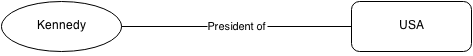
\includegraphics[width=10cm]{ken.png}
               \caption{triplet ''Kennedy''}

\end{figure}
\subparagraph{}
Le premier triplet n'a pas une sémantique valide que en tenant compte du triplet suivant~: 
\begin{figure}[H]
        \centering
                \centering
                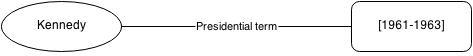
\includegraphics[width=10cm]{presidterm.png}
               \caption{triplet presidential term ''Kennedy''}

\end{figure}
\subparagraph{}
On vise plutôt à annoter les triplets (s,p,o) avec une étiquette temporelle qui précise la validité de ce terme dans un cadre logique qui appartient au monde réel où en dehors de ce cadre, on peut dire que ce triplet RDF n’est pas valide et qu’on ne peut pas l’utiliser.
\subsection*{Sources des données DBpedia}
\paragraph{}
Les faits temporels extraites de Wikipedia consiste en deux phases principales : extractions des données semi-structurées(tableaux, infoboxes) et l’extraction depuis le texte wikipédia.
\subsubsection*{Texte Wikipedia}
\paragraph{}
On cherche à extraire les informations temporelles qui ont un contexte de validité lié à un fait à partir des données textuelles des pages de Wikipedia. 
Par exemple sur la page de John Fitzgerald Kennedy, on retrouve~:
\newline
Kennedy a visité Berlin Ouest le 23 Juin 1963.
\subparagraph{}
On veut extraire les ressources en donnant une nouvelle structure pour mieux présenter leur contexte de validité temporelle.
\subsubsection*{Infobox Wikipedia}
\paragraph{}
Les infoboxes : Contiennent généralement les informations les plus importantes des entités décrites dans l’article. Par exemple dans l’infobox de “Kennedy” l’ancien président des États-Unis sur wikipédia on trouve la date d’élection, le prédécesseur du président, la durée du mandat, etc…
\newline
Chaque infoBox a un type particulier comme: évènement historique, élection, compétition ect…
\begin{figure}[H]
        \centering
                \centering
                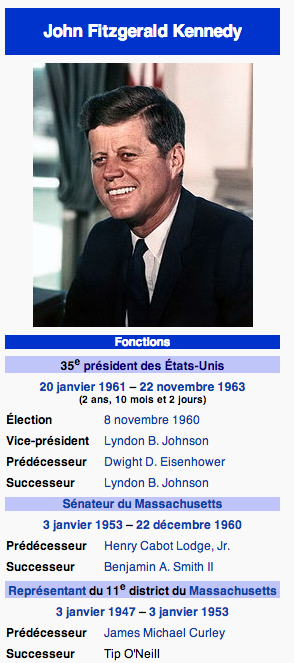
\includegraphics[width=5cm]{kennedy.png}
               \caption{Info Box Wikipedia ''Kennedy''}

\end{figure}
\subsubsection*{Tableau}
\paragraph{}
Dans les tableaux “Wikipedia” figurent des informations temporelles plus structurées et plus faciles à extraire, qu’on cherche à récupérer.
\subparagraph{}
Vous trouverez ci-dessous des informations sur les anciens précidents des États-Unis.
\begin{figure}[H]
        \centering
                \centering
                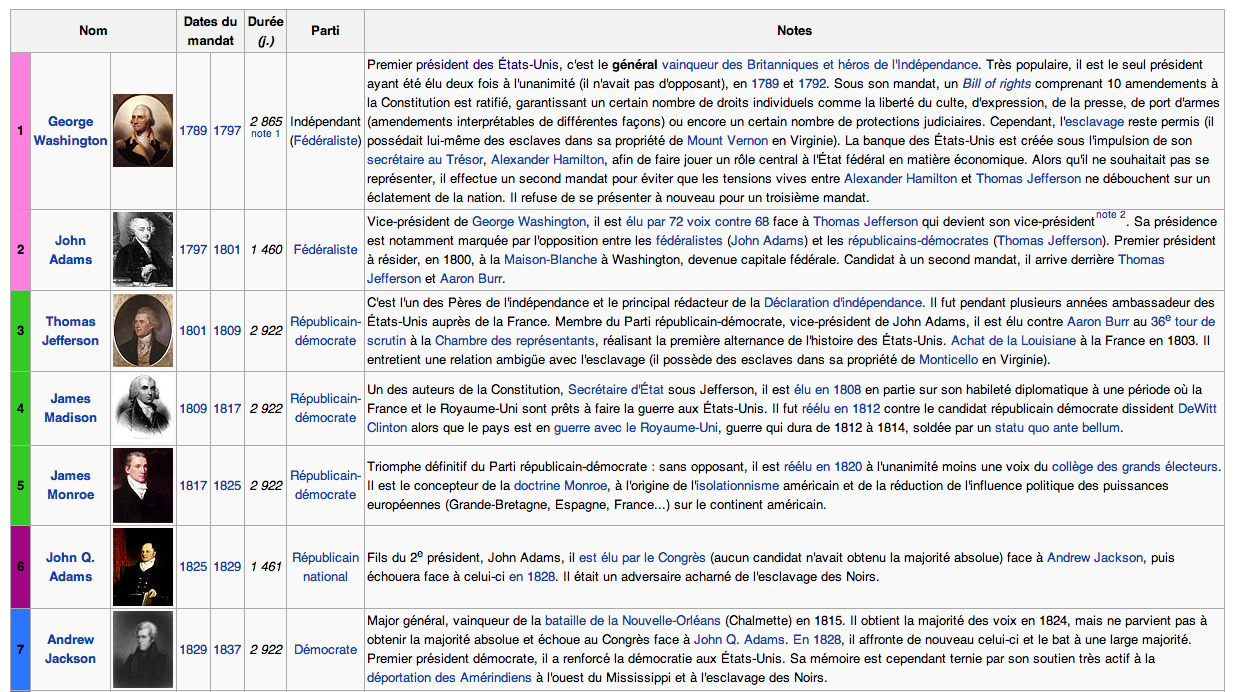
\includegraphics[width=14cm]{tableau.png}
               \caption{Exemple de tableau Wikipedia}

\end{figure}
\subsubsection*{Wikidata}
\paragraph{}
Sur la page wikidata, liée au contenu de la page wikipedia de Kennedy, on a intérêt à extraire les informations temporelles.
\begin{figure}[H]
        \centering
                \centering
                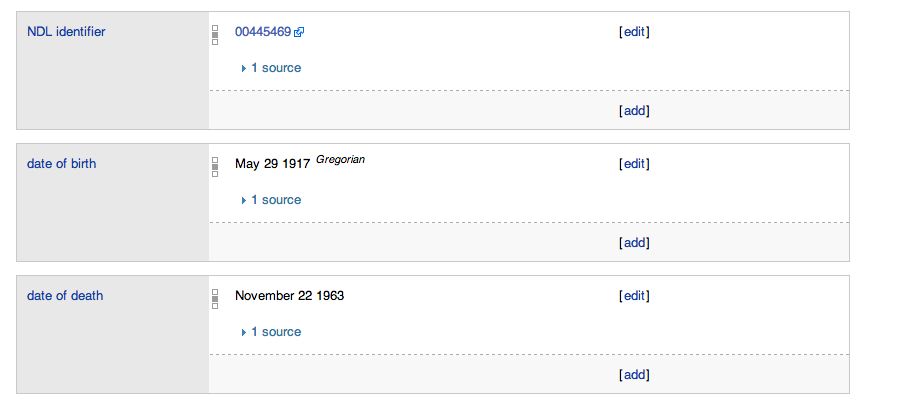
\includegraphics[width=14cm]{wikidata.png}
               \caption{Exemple Wikidata}

\end{figure}
\subsubsection*{Historique des pages wikipedia}
\paragraph{}
On souhaite, si c’est possible, extraire des informations temporelles relatives à l’historique de modifications des pages de wikipedia. Car, il se trouve qu’il y on a beaucoup d’informations liées à cet historique.
\subsubsection*{Résumé}
\paragraph{}
Il s'avère que beaucoup de points du temps dont liées à plusieurs sources d’information évènementielle; on cherche à extraire ces informations afin de les mettre sous une forme plus adéquate.
\subsection*{Notre modélisation}
\paragraph{}
Modèle quaternaire : un modèle qui capte la base du fait avec un indice temporel.
\newline
<politician> served as <politician office> from <date> to <date>
\newline
f1: Kennedy holdsPoliticalPosition PresidentOfUSA 
\newline
f2:f1 startedOnDate 
\newline
f3:f1 endedOnDate
\newline
HappenedDate est utilisée pour dire que le fait est valide que dans ce point du temps.
\begin{figure}[H]
        \centering
                \centering
                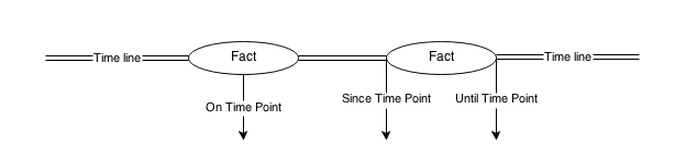
\includegraphics[width=10cm]{timeline.png}
               \caption{Event Time Line}

\end{figure}
\subparagraph{}
Pour surmonter ce problème et exprimer la validité temporelle d’un triplet RDF d’une manière à la fois intelligente et lisible par la machine; on souhaite rattacher au triplets valides que dans une plage temporelle bien précise une étiquette temporelle adéquate.
\newline
Exemple~:
\begin{figure}[H]
        \centering
                \centering
                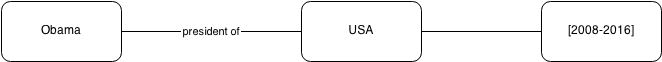
\includegraphics[width=10cm]{obamaQuad.png}
               \caption{Modélisation quadruplet}

\end{figure}
\subparagraph{}
On s'intéresse au format N-Quads qui est un standard w3c basé sur la forme N-Triples. L’avantage est qu’il se distingue par la possibilité d’encoder des graphes multiples.
Les quadruplets vont être formalisés de la manière suivante~:
\newline
$<s,p,o,[t1,t2]>$, un sujet, prédicat, objet avec une intervalle de temps.
\newline
$<s,p,o,t>$, de même avec un point de temps $t$.
\section*{Analyse temporelle}
\subsection*{Représentation}
\paragraph{}
Les informations temporelles peuvent avoir des repèsentations différentes~: 
\begin{itemize}
\item Un évènement `` Je vous propose un rendez-vous $demain$ pour parler de ma plateforme PiSharing``. \item Une connaissance `` Jacques Chirac est le président de la république Française `` \textbf{ mais quand ?}.
\end{itemize}
\subsection*{Ambiguïtés temporelles}
Le présent par exemple peut avoir plusieurs sens ou contextes : présent de narration, présent de généralité, présent qui réfère au futur proche, etc...
\subparagraph{}
Les signaux temporelles sont ambigus~: réunion de 14h à 16h, il court pour rattraper le temps, tu tournes après la rivière, etc…
\subparagraph{}
La plupart des expressions sont floues~: il y a deux ans, chaque deux semaines, j’arrive dans deux secondes, etc...
\paragraph{}
L’analyse du temps s’inscrit dans la compréhension globale des textes, et des évènements auxquels on fait référence dans ce texte. 
\newline
Modalité~: l’équipe de France voulait gagner la coupe du monde en 2006. 
\newline
Anaphore~: cela pourrait avoir lieu dans les éditions suivantes.
\subparagraph{}
Les évènements décrits (et que l’on souhaite fixer temporellement) peuvent être: duratifs ou ponctuels/accomplis ou inaccomplis. 
\subparagraph{}
De même pour les dates qui peuvent être~: Date absolue ``le 18 mars, c'est mon anniversaire``; Date relative par rapport au moment de l’énonciation~: `` il y a deux ans ``. Pour la durée~: Durée absolue `` durant 2 ans ``; Durée relative~: `` depuis un an ``.
\subparagraph{}
On trouve aussi~: Expression de fréquence `` tous les ans, le vendredi 13 ``, Expression plus complexe `` après la Révolution Tunisienne ``.
\subsection*{Résumé}
\paragraph{}
Dans l'encyclopédia libre Wikipedia, il se trouve qu’il y a beaucoup d’informations temporelles; qu'on risque de retrouver par la même occasion dans DBpedia. Dans cette étude on va plutôt essayer d’extraire des dates saillantes en fonction de leurs sémantiques évènementiels.
\section*{Proposition}
\subsection*{Introduction}
\paragraph{}
L'annotation d'un triplet RDF est une façon d'ajouter des metadonnées à un triplet RDF pour décrire la validité temporelle, une restriction spatiale, ect...
\newline
\textit{Comment on utilise les annotations temporelles ?}
Sur le site sig.ma\footnote{http://sig.ma/} créer par\textit{the digital enterprise research institute in Ireland}, la plateforme fournit un moteur de recherche par mot clé qui permet de récupérer des images et des textes accessibles par des annotations RDF, ainsi que d'une liste d'URI synonymes correspondant à la clé de recherche et des liens vers des sources Web contenant des données RDF pertinentes.
\subsection*{Schéma de modélisation}
\paragraph{}
Notre première modélisation a été conçu de la manière suivante :
\newline
Tout d’abord, et à partir des différents sources d’informations on veut récupérer les informations temporelles dans leurs contextes sémantiques à l’aide de nos différents extracteurs implémentés. 
Ensuite, les mettre dans un ensemble de fichiers comme le montre le schéma ci-dessous.
\begin{figure}[H]
        \centering
                \centering
                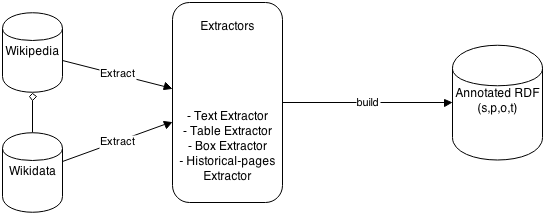
\includegraphics[width=10cm]{modelisation.png}
               \caption{Modélisation générale}

\end{figure}
\subparagraph{}
Certes, on peut créer des “patterns” partons ou motifs à travers les faits temporels dans la base de connaissances mais on cherche ici à extraire les informations des textes et des données semi-structurée afin de leur trouver une autre structure plus adéquate (tel un triplet annoter ou bien un quadrupet).
\subsection*{Démarche}
\paragraph{}
Au début, nous avons commencé par une procédure d’extraction des faits dans les sources d'information XML de wikipédia. Nous avons réussi à extraire des fais mais nous avons rencontré des problèmes relatives à la taille du dumps wikipédia/wikidata et au fait de relier ces informations temporelles au bon contexte du triplet qu’on veut annoté.
\subparagraph{}
Ce fait nous a amené à chercher une autre solution que celle choisi au départ.
Nous avons trouvé une solution plus intelligente pour former les quads ou des triplets annotés à partir des sources de données DBpédia.
\subparagraph{}
Sur le site de DBpedia, nous avons étudié les deux formats du dumps JSON et CSV afin de voir la structure des informations.
Suite à nos observations nous avons décidé de manipuler les fichiers CSV pour voir la logique et la structure de ces informations.
\subparagraph{}
Nous cherchons à former les quadruplets à partir des faits existants dans DBpedia.
Dans cette dernière, on trouve des faits temporels et d’autres faits relié à leurs contexte.
\subparagraph{}
Une liste des faits sera proposer en output et un expert sera placer pour juger la validité des données trouvées par notre algorithme sous forme de résultats labellisés en premier temps puis d'enregistrer les ressources dans des fichiers de quadruplets RDF classés selon des catégories bien spécifiques.
L’expert peut sélectionner la liste des indicateurs $tokens$ temporels misent par défaut dans le code de l’application, ajouter des indicateurs à la liste existante ou bien introduire une nouvelle liste d’indicateurs.
Sachant que plus on introduit des indicateurs temporels, plus on aura des couples.
\subparagraph{}
Nous avons testé notre algorithme avec les deux indicateurs $YEAR$ et $DATE$.
L'algrithme cherche à trouver une liste de couple de faits temporels et faits reliés possible qui seront les entrées d'une requête $SPARQL$.
\subparagraph{}
L'expert intervient pour juger la validiter des résultats trouvés.
Un seul output valide peut donnée un ou plusieurs résultats ''des triplets annotés''.
Nous avons défini une base SPOTbase ($Subject$, $Predicate$, $Object$, $Time$) qui contient les quadruplets extraits par catégorie.
\subparagraph{}
Nos algorithmes manipulent des ressources DBpedia afin de les mettre sous un autre forme valide dans le temps et tout en gardant une sémantique correcte. 
\subsection*{Procédure}
\paragraph{}
Notre proposition consiste à extraire des faits temporels de la forme suivant :
\newline
$***Entity*with*TemporalToken***$ puis de chercher d’autres propriétés reliées à ces faits temporels $***Entity*with*OtherWord***$.
On donne la main à un expert pour choisir un couple de faits puis de valider les résultats générer automatiquement par notre algorithme afin de mettre en place les quadruplets dans la base SPOTbase. 
\subsubsection{Étapes}
\paragraph{}
La première étape consiste à trouver tout les propriétés et les stockers dans un fichier pour les exploités comme une base de faits.
\newline
Algorithme : getProperties(propFile)			
\newline
writer<=bufferWriter(propFile)
\newline
resultSet<=queryExecution(query)                         
\newline
writeProperties(resultSet,writer)				
\paragraph{}
L'étape suivante consiste à trouver la liste des faits temporels à partir de la liste d'indicateurs mise par défaut ou introduite par l'expert.
\newline
Algorithme : getTemporalFacts(tToken, propFile) 			
\newline
buff <= ReadFile(propFile)    			
\newline
tf<=ListFacts(buff,tToken) 				
\newline
removeDuplication(tf)
\paragraph{}
La procédure d'extraction continue pour extraire les faits reliés, à partir de la liste de faits temporels trouvés. On cherche à extraire un nombre maximal de faits reliés pour avoir plus de résultats.
\newline
Algorithme : findCouple  			
\newline
getPairListAtt(file,tf)
\newline
listToken<=findTokens(tf,tp)   
\newline      
hashSet<=getHashSetList(listToken) 
\newline
printList(hashSet)				
\paragraph{}
Le choix de l'expert consiste à selectionner le couple de faits pour lancer automatiquement l'algorithme qu'on a conçu permettant de récuperer les informations nécessaires pour former des triplets annotés.
\newline
Notre besoin se résume comme suit :
\newline
if ($x$ propTemp $y$) and ($x$ prop*** $z$) then
\newline
($x$ prop*** $z$) $y$ with ($y$ is the temporal annotation)
\subparagraph{}
Les résultats de la requête labelisés seront affichés dans un $TextArea$ à l'expert en premier lieu puis ils peuvent être stocker dans un fichier sous forme de quadruplets RDF.
Les quadruplets annotés seront sauvegardés dans le fichier nommé par l'expert dans le dossier de la base de donnée SPOTbase.
\subparagraph{}
Pour obtenir des quadruplets on a essayé de trouver des propriétés qui se rencontrent avec une procédure automatique mais le choix de l’expert et la validation des résultats à toujours important. Cela peu avoir un impacte déterminant sur le reste du travail et la nature des résultats.
\subsection*{Récapitulatif}
\paragraph{}
Nous avons construit à partir de la base de connaissance DBpedia une autre base de  triplets temporairement annotés qu’on a nommé SPOTbase.
SPOTbase contient une liste de fichiers dans lesquels on a des quadruplets ($subject$, $predicat$, $object$, $time$) avec une sémantique correcte. 
\subparagraph{}
Par la suite, nous avons choisi d’extraire des propriétés temporelles liées à une liste d'indicateurs pour tourner nos algorithmes.
\subparagraph{}
Une première étape consiste à extraire tous les faits DBpedia et les stockés dans un fichier puis la seconde consiste à proposer une liste de couple de faits à l’expert.
\subparagraph{}
Dans l’étape suivante on va interroger DBpedia en utilisant une requête SPARQL qui retourne trois variables ($x$,$y$,$z$) le choix de l’expert est primordiale pour valider les résultats trouvés.
Enfin les ressources formées en quadruplets seront stockés dans SPOTbase.   
\newline
( $X$ prop\_liée $Y$ ) annoté avec $Z$.
\subparagraph{}
Notre nouvelle approche à la particularité de manipule directement les ressources de DBpedia.
Des anciens travaux de recherches ont évoqué la même problématique en essayant de rattacher des annotions aux données de wikipedia alors que dans notre étude nous cherchons à regrouper des propriétés des triplets existants afin de former des triplets annotés.





		


 

\bibliographystyle{alpha}
\bibliography{Biblio.bib,w3c.bib}
\end{document}